\section{Swarm Algorithm Validation}

To measure the effectiveness of the swarm algorithms, I have implemented a surveillance scenario within the simulator. The scenario consists of a 3km x 3km search area \ref{fig:swarm_validation_area}, placed in anchorage zone for Gdańsk harbour. The search area is populated with 5 vessels, including a mix of cargo ships and tankers The swarm is tasked with patrolling the area. Whole area is divided into 300mx300m grid cells, and the swarm must continuously patrol the area, visiting each cell at least once. The swarm is also required to avoid collisions with the vessels, which are moving according to recordings of real AIS traffic in the area. The swarm is also required to avoid collisions with each other. The performance of the swarm is measured in terms of the time taken to achieve complete coverage of the search area. The results of this validation scenario are presented below.

\vspace{1cm}
During the test, drones desired speed was set to 10 m/s, which is a very fast speed for a USV, but could be achieved in real life during very calm sea conditions. Such a speed would also very fast drain the battery, but it could be used during emergency situations, such as search and rescue operations, where time is of the essence. In the two tests, swarm consisted of 18 drones and 9 drones.


    \begin{figure}[htbp]
        \centering
        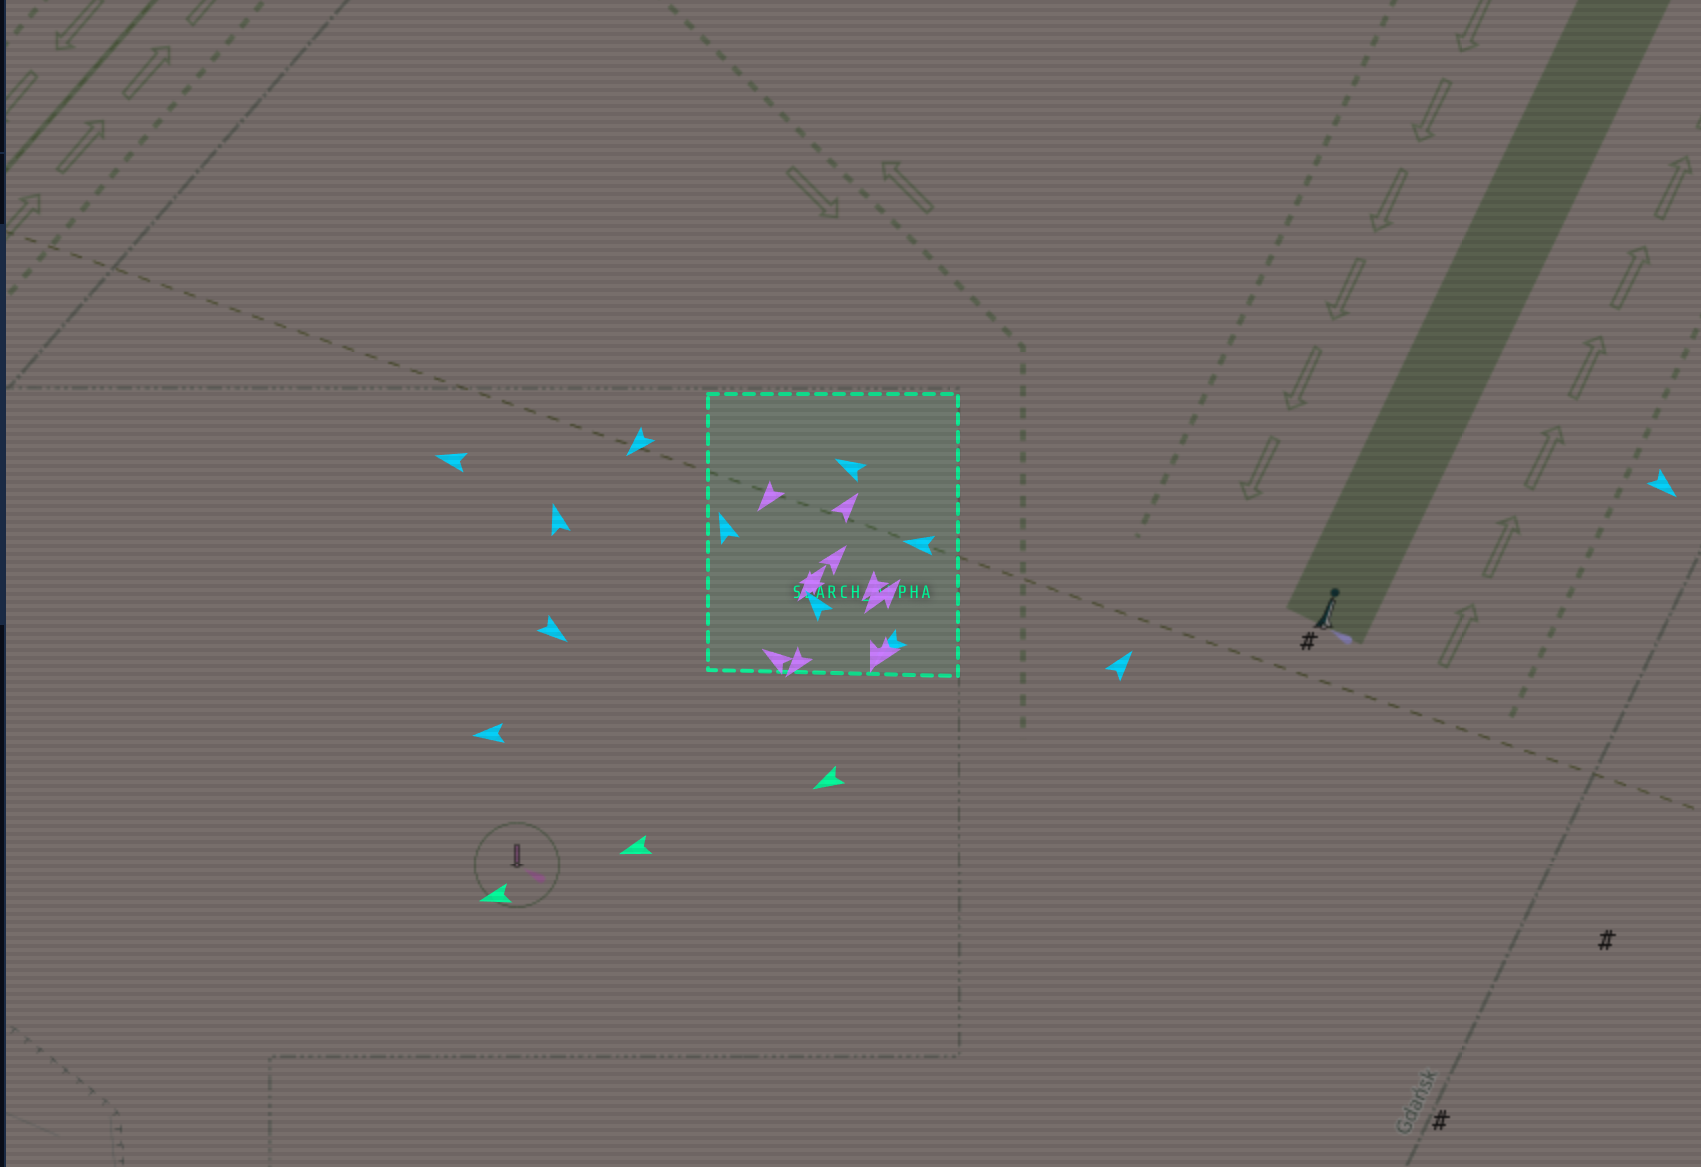
\includegraphics[width=0.9\textwidth]{images/validation_zone.png}
        \caption{ Search zone for swarm validation. The green dotted square represents the 3km x 3km search area, while the blue dots represent the positions of the 5 vessels and purple dots represent the positions of the drones.}
        \label{fig:swarm_validation_area}
    \end{figure}


    First plot \ref{fig:swarm_visited_cells} shows the percentage of area visited by the swarm over time. The swarm achieves complete coverage of the search area in approximately 45 minutes, which is a reasonable timeframe for a real-world surveillance mission. The plot also shows that the swarm is able to maintain a steady rate of coverage throughout the mission, indicating that the algorithms are effective at coordinating the drones and avoiding collisions with the vessels and each other. 


    \begin{figure}[H]
        \centering
        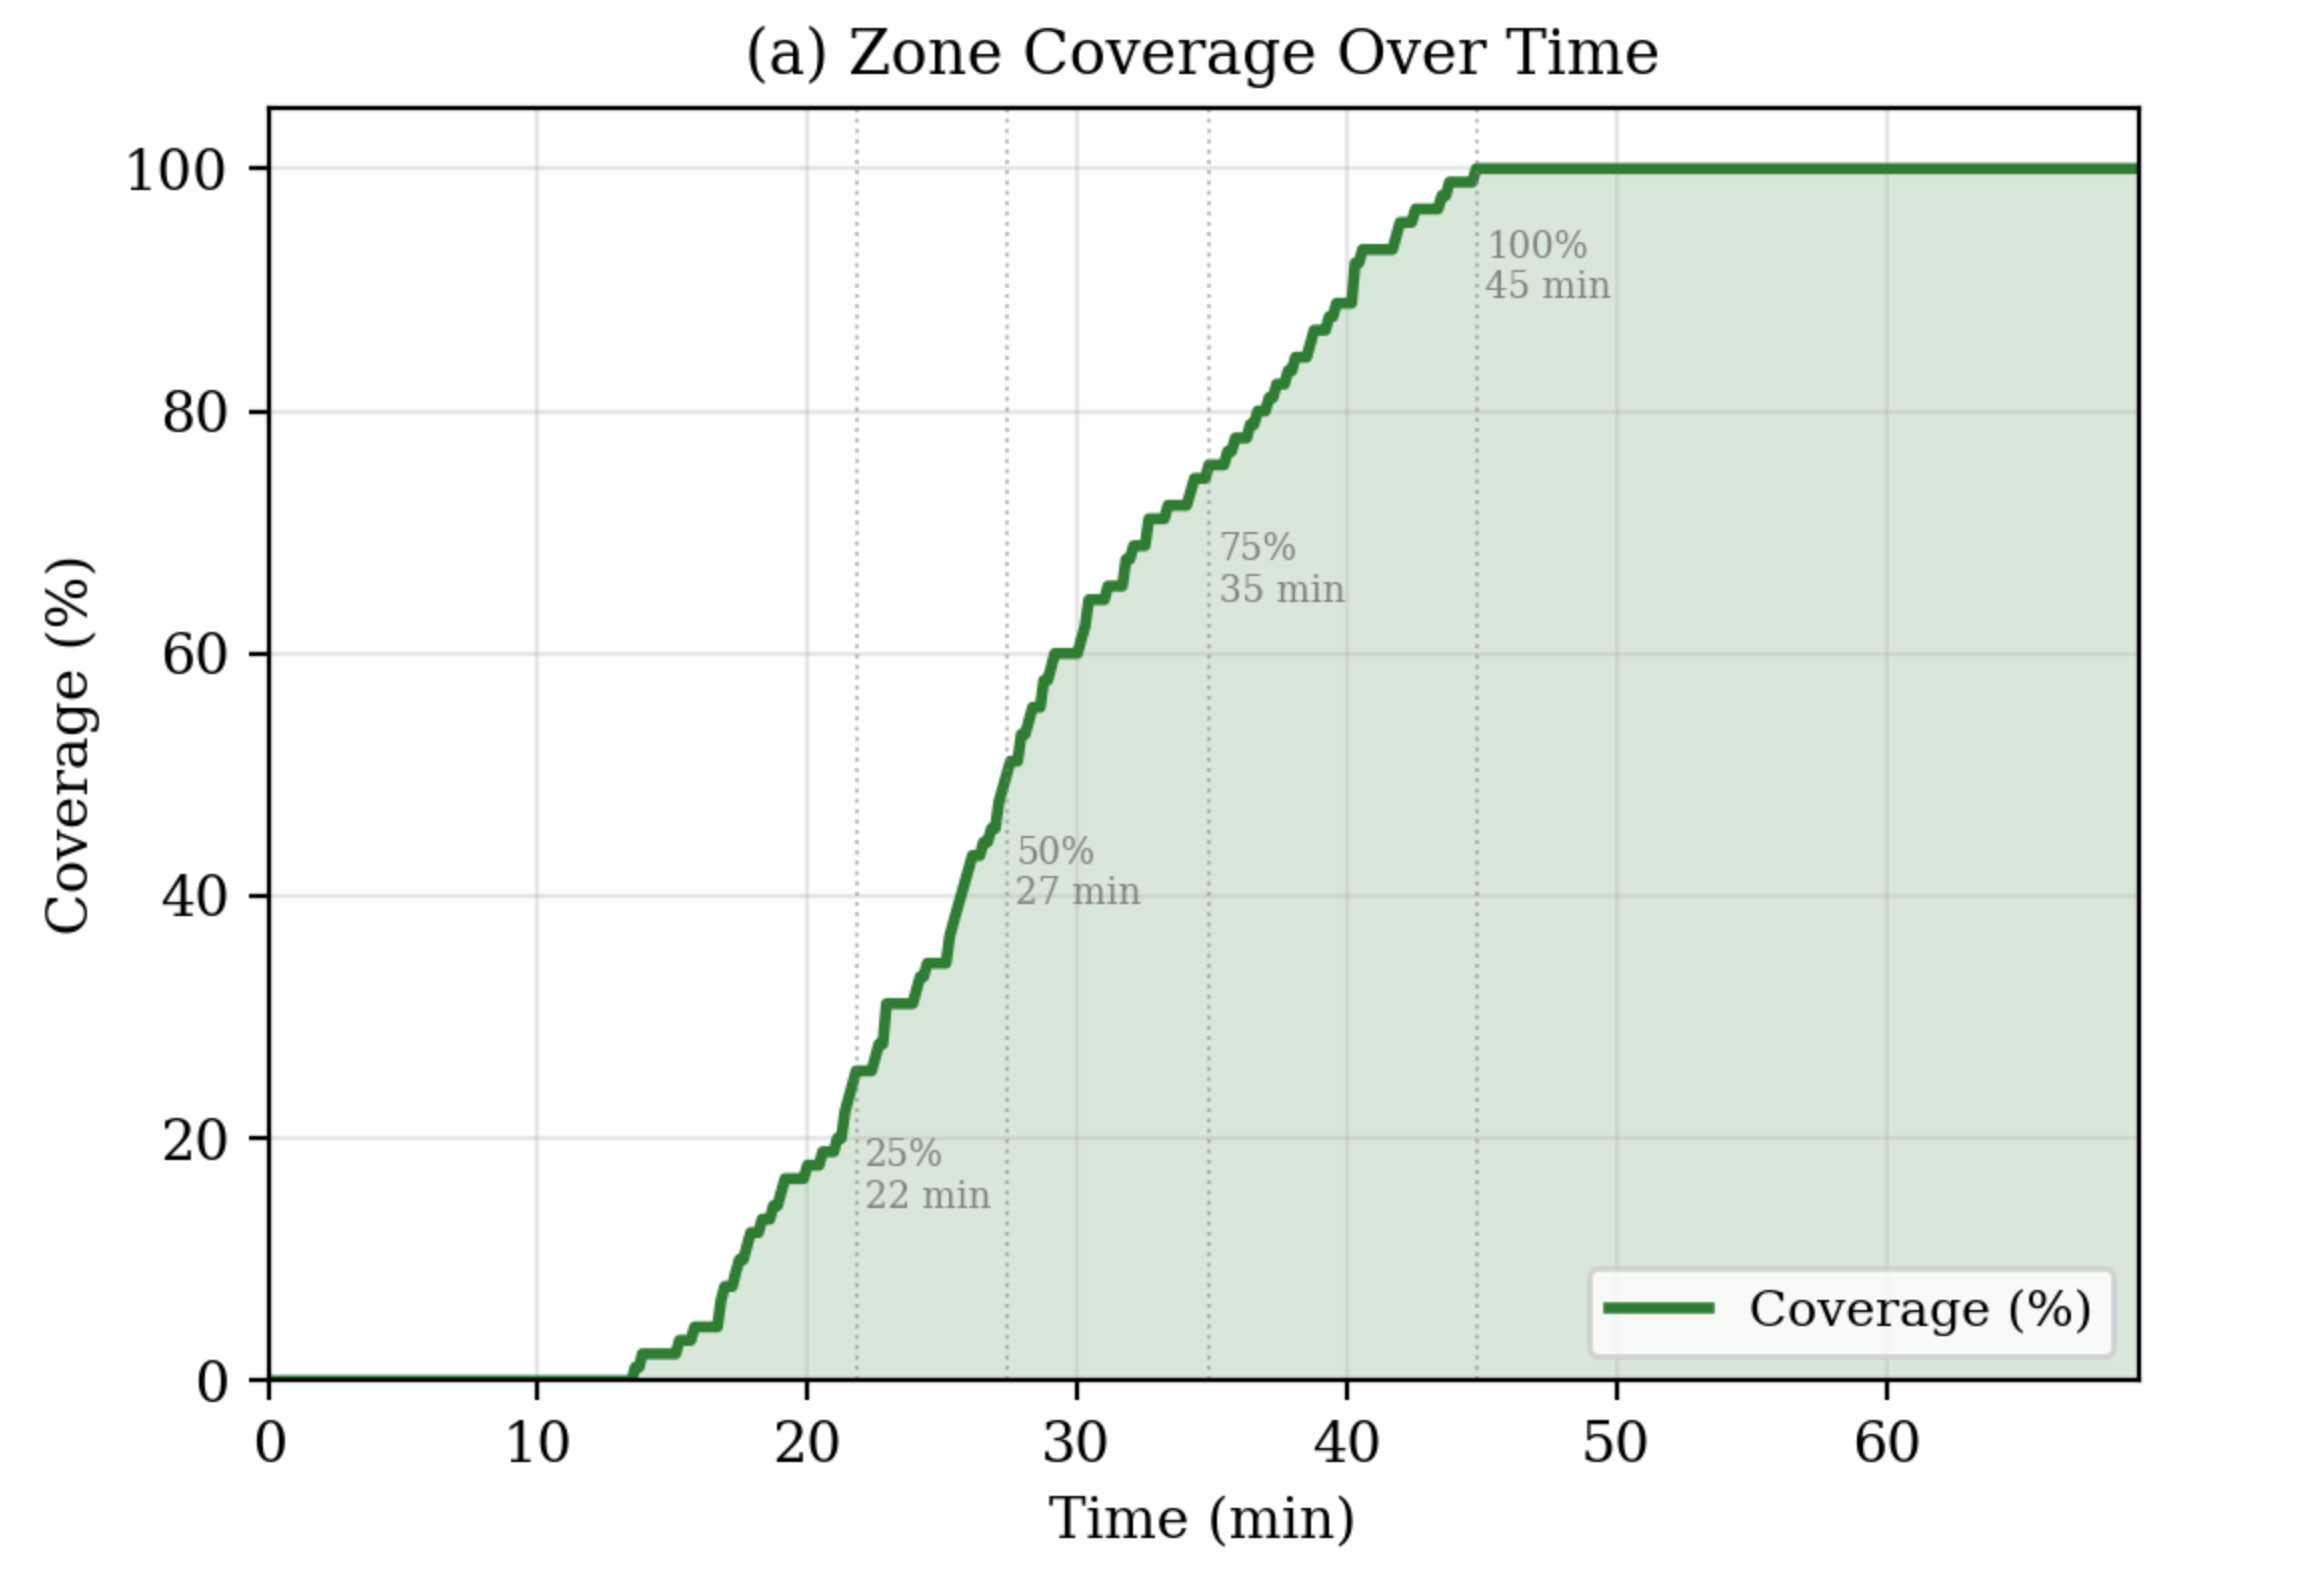
\includegraphics[width=0.9\textwidth]{images/18UAVs_coverage.png}
        \caption{Percentage of grid cells visited by the swarm during validation, for a swarm of 18 drones. The swarm achieves complete coverage of the search area in approximately 45 minutes.}
        \label{fig:swarm_visited_cells}
    \end{figure}



    Second plot \ref{fig:swarm_grid_plot} shows the grid cell visitation plot for the swarm validation scenario. Drones entered the search area from the bottom right corner and propagated first towards left and then upwards, following the grid-based search pattern. It is well visible that some dots are darker than others, which indicates that some cells were visited multiple times. This is a result of the collision avoidance algorithm, which causes drones to not always follow the optimal path to the next unvisited cell, but instead take detours to avoid collisions with vessels and other drones. Overall, the plot shows that the swarm is able to effectively coordinate their movements and achieve complete coverage of the search area while avoiding collisions.



    \begin{figure}[H]
        \centering
        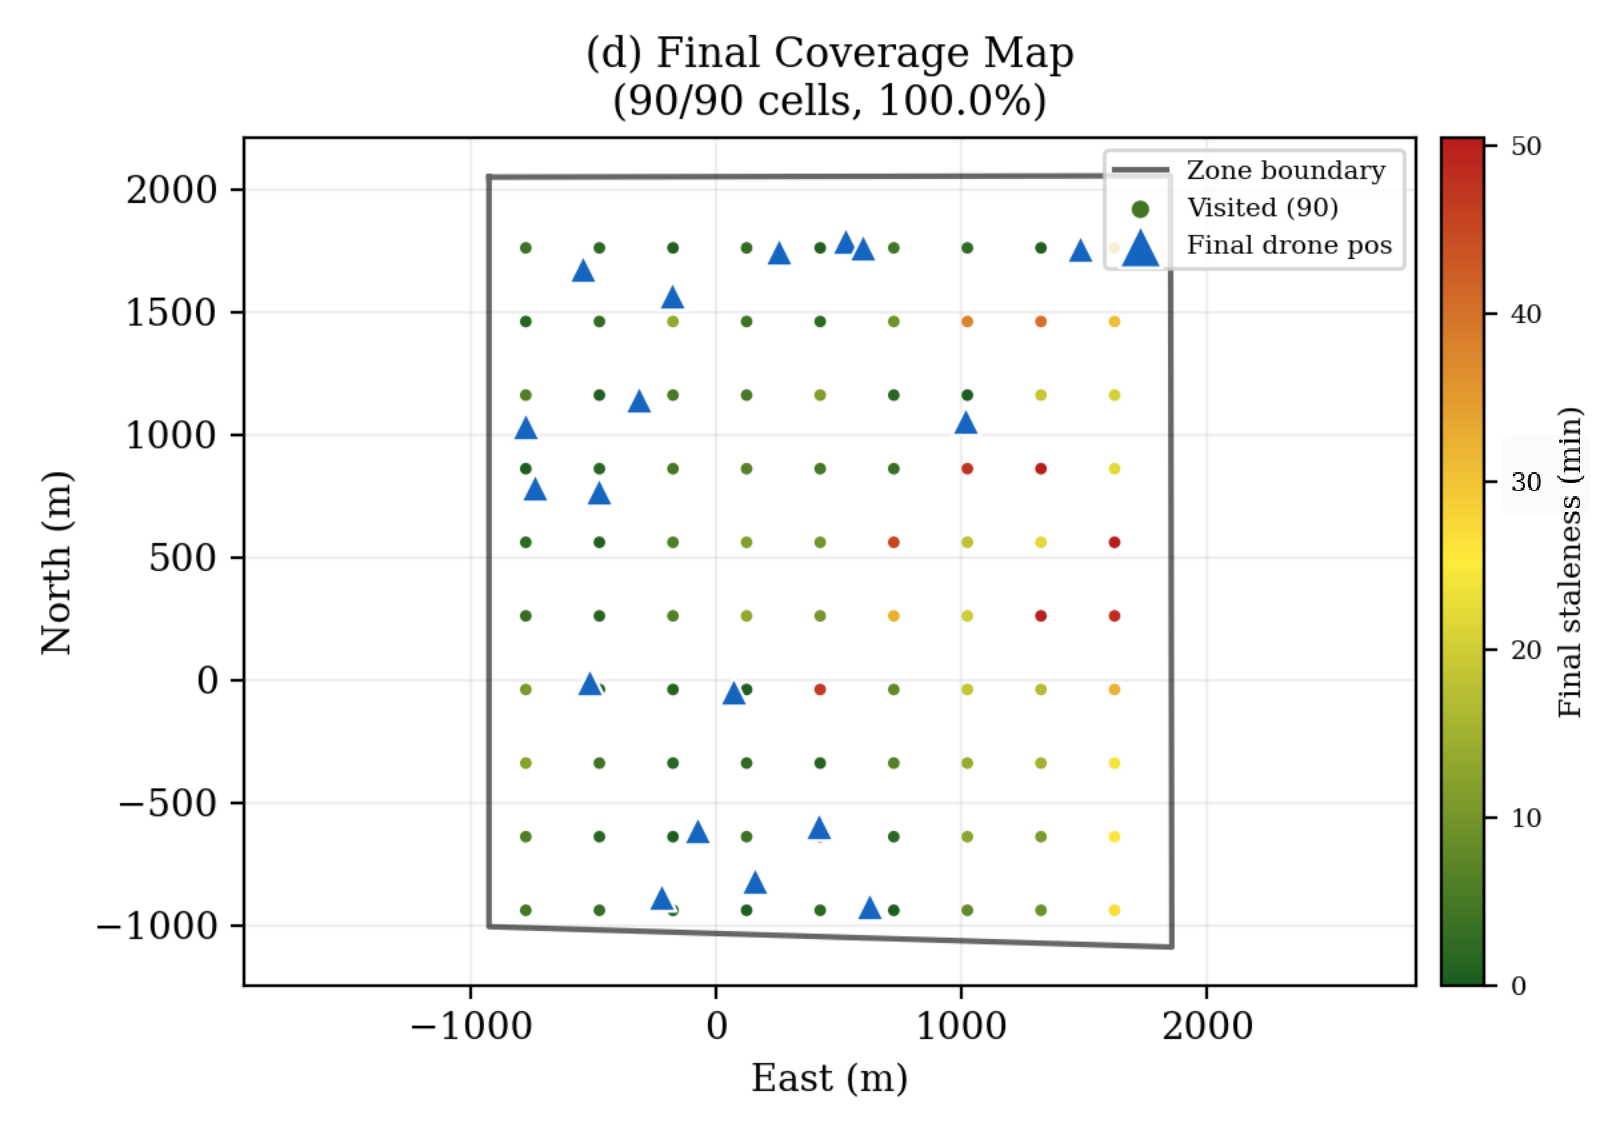
\includegraphics[width=0.9\textwidth]{images/18UAVs_grid_coverage.png}
        \caption{Grid cell visitation plot for the swarm of 18 drones. Each dot represents a grid cell, with color indicating the time of last visitation. }
        \label{fig:swarm_grid_plot}
    \end{figure}



Third plot \ref{fig:18UAVs_between_drones_distance} shows the inter-drone distance plot. The plot shows that the swarm is able to maintain safe distances between drones, with no instances of collisions. The plot also shows that the mean distances in a begining of the mission are increasing. That shows that the drones are spreading out to cover the area more effectively, which is a desirable behaviour for a search mission.



\begin{figure}[H]
    \centering
    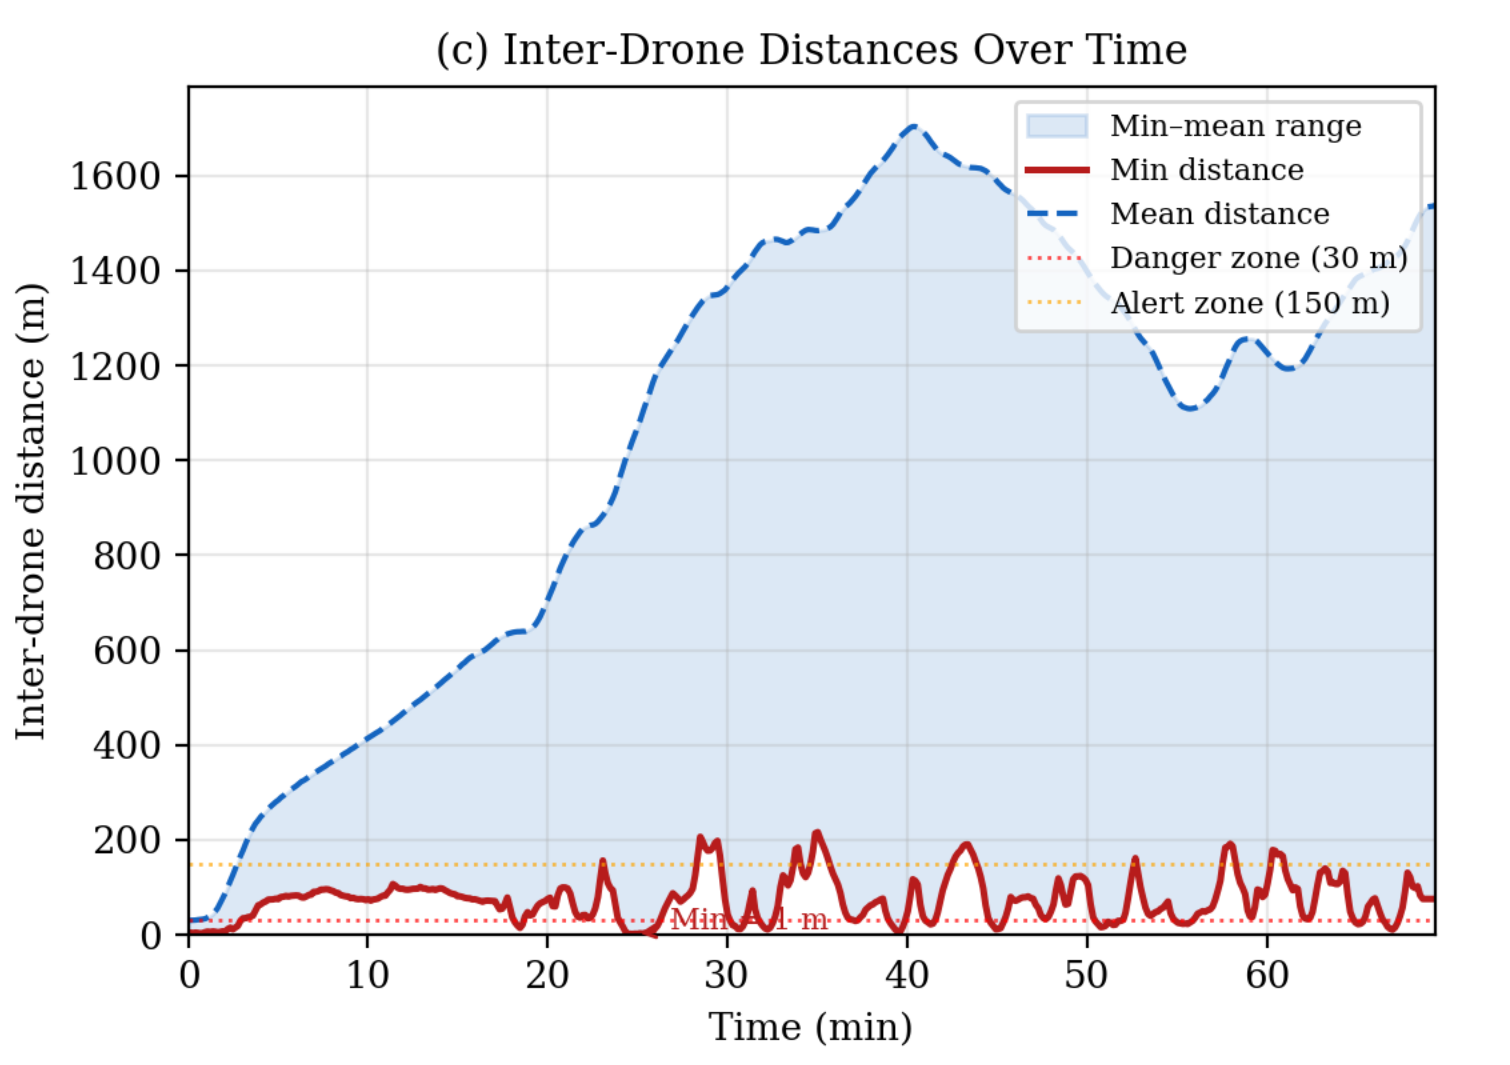
\includegraphics[width=0.9\textwidth]{images/18UAVs_inter_drones.png}
    \caption{ Inter-drone distance plot for the swarm validation scenario.The plot shows that the swarm is able to maintain safe distances between drones, with no instances of collisions or near-collisions.}
    \label{fig:18UAVs_between_drones_distance}
\end{figure}






To compare that data I have also run the same scenario with a swarm of 9 drones, which is half of the original swarm size. The results are shown in the plots below. The first plot \ref{fig:swarm_visited_cells_9} shows that the swarm of 9 drones achieves complete coverage of the search area in approximately 53 minutes, which is not significantly longer than the time taken by the swarm of 18 drones. That is probably due to the fact that the search area is relatively small, and the drones are wasting lot of time on collision avoidance, which limits the benefits of having more drones in the swarm. That is also visible in third plot \ref{fig:9UAVs_between_drones_distance}, which shows that the mean inter-drone distances are higher for the swarm of 9 drones, which indicates that the drones are less likely to collide with each other, but also more likely to cover the area effectively. Overall, the results show that the swarm algorithms are effective at coordinating the drones and achieving complete coverage of the search area, even with a smaller swarm size. However, it is important to note that the performance of the swarm may vary depending on the specific scenario and environmental conditions, and further testing is needed to fully evaluate the algorithms under a wider range of conditions.

    \begin{figure}[H]
        \centering
        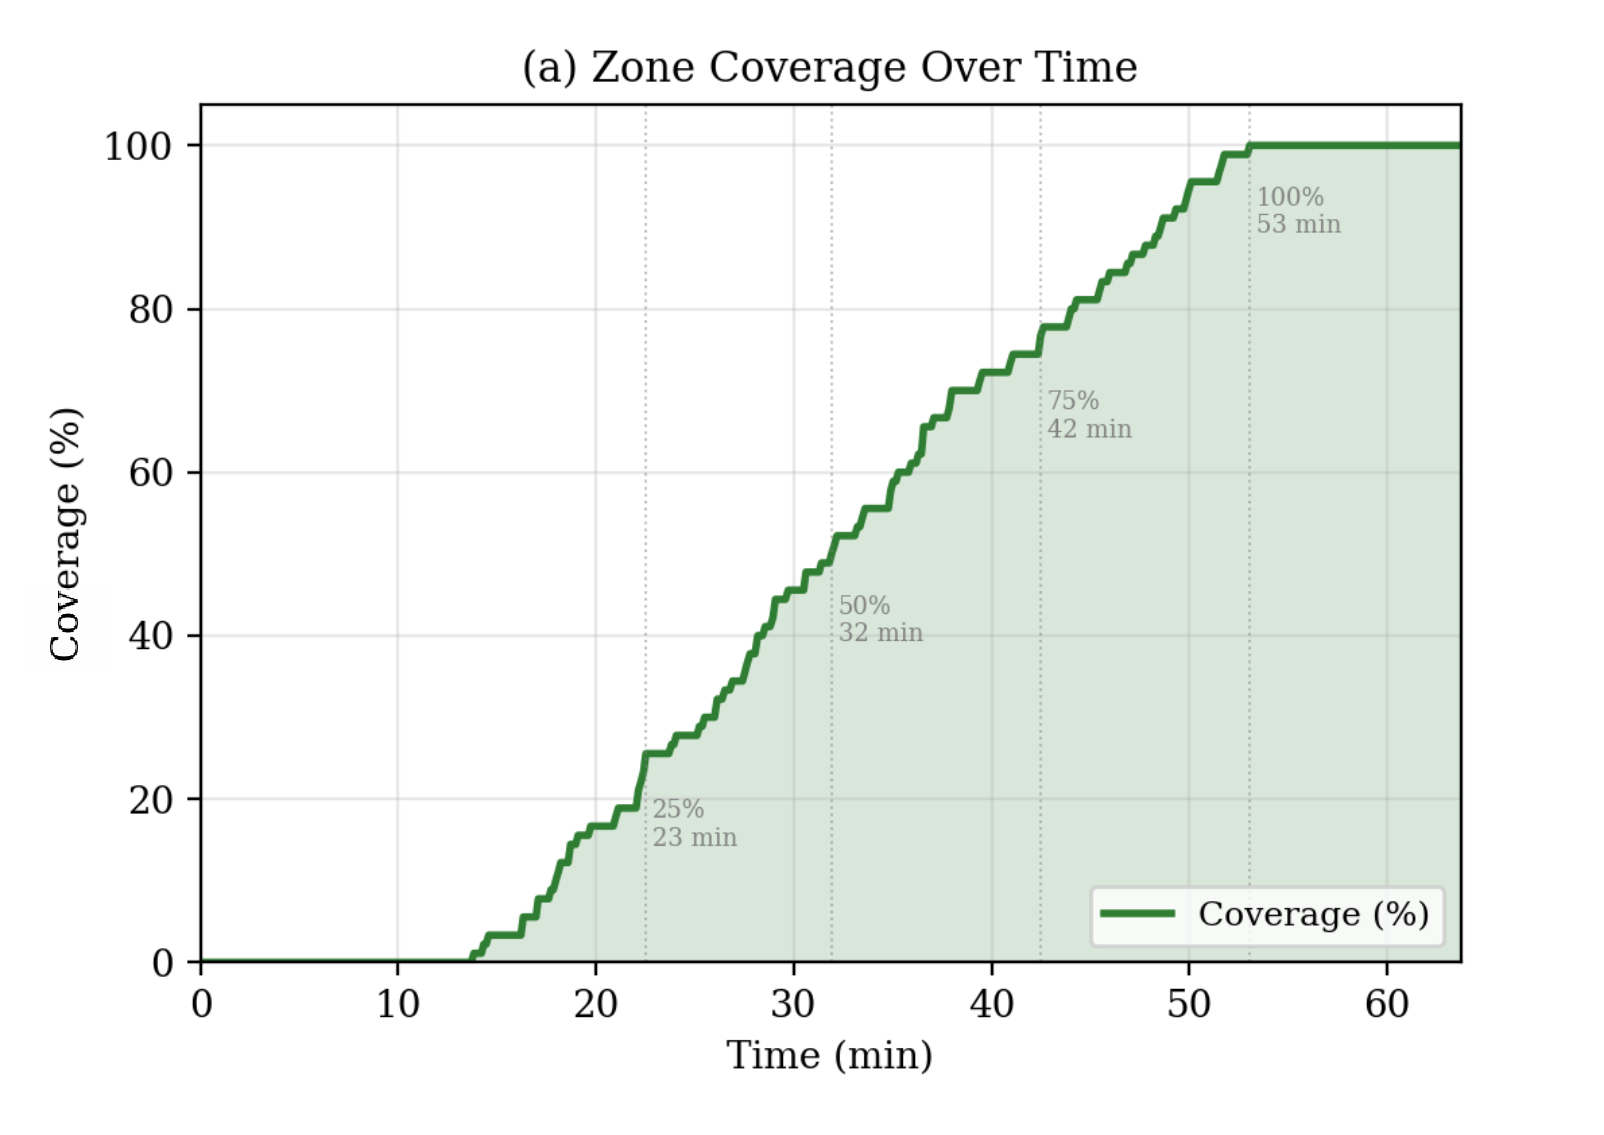
\includegraphics[width=0.9\textwidth]{images/9UAVs_coverage.png}
        \caption{Percentage of grid cells visited by the swarm during validation, for a swarm of 9 drones. The swarm achieves complete coverage of the search area in approximately 53 minutes.}
        \label{fig:swarm_visited_cells_9}
    \end{figure}


    \begin{figure}[H]
        \centering
        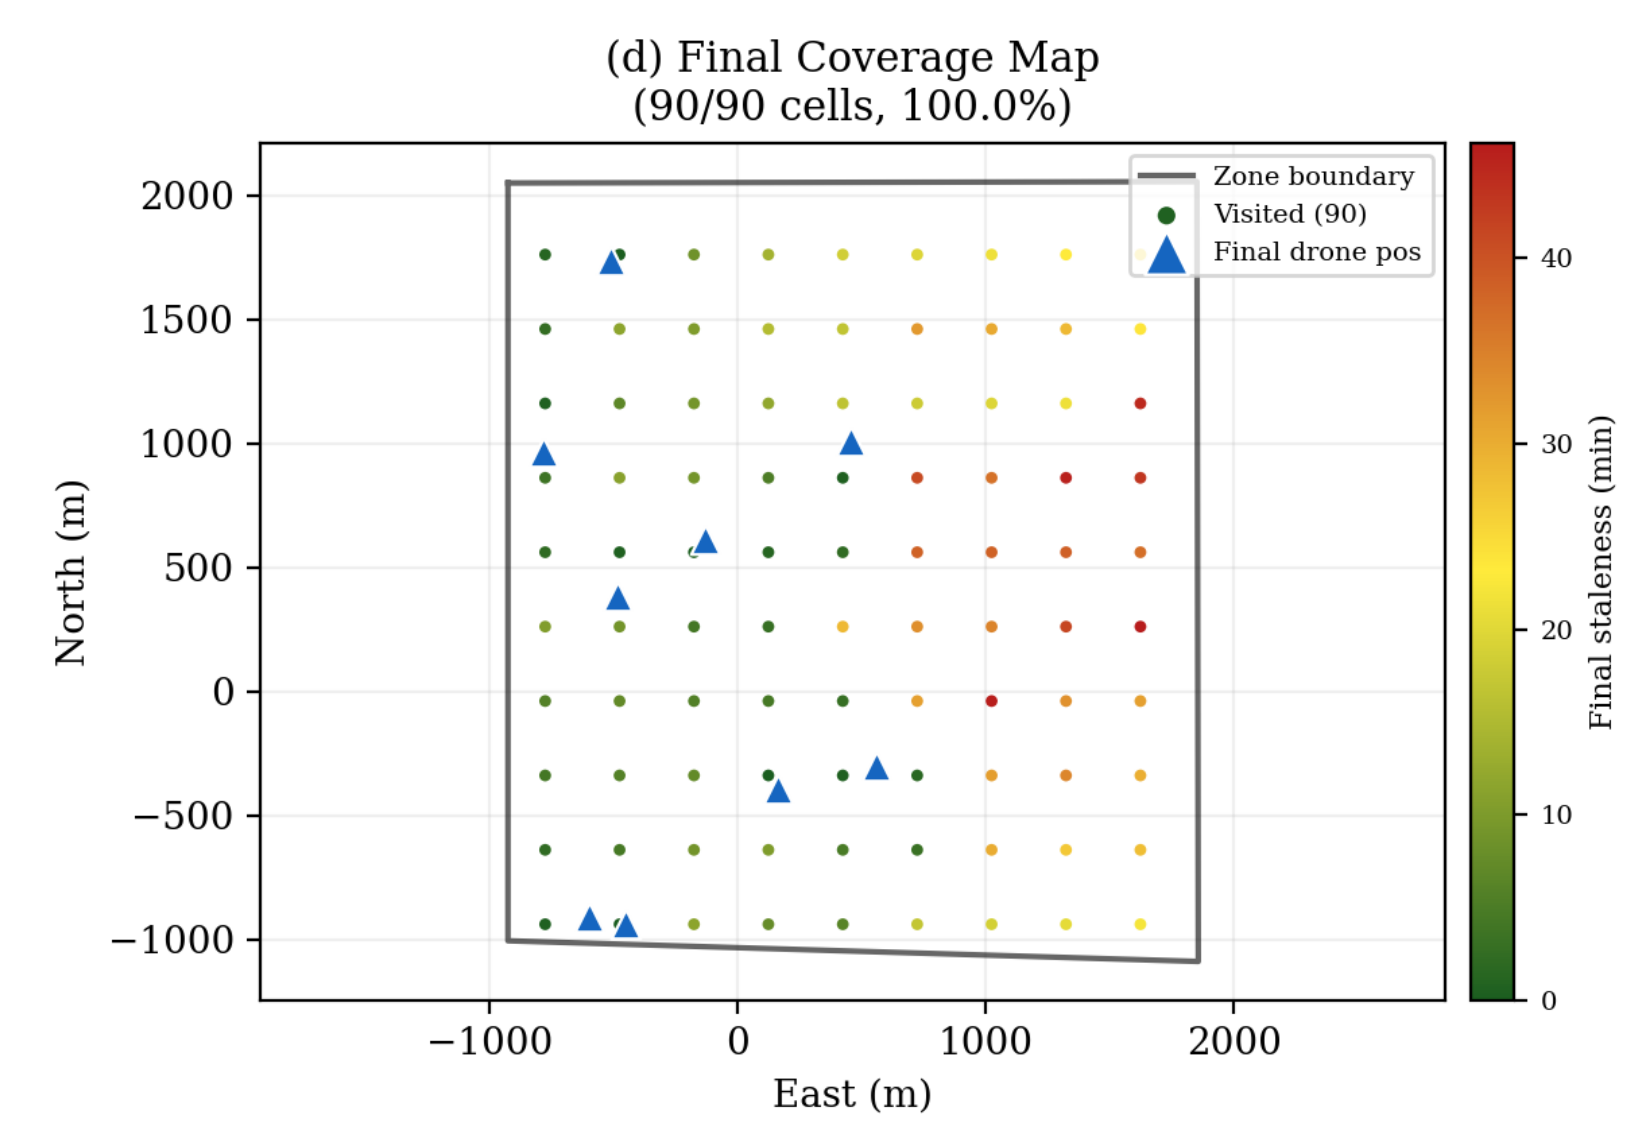
\includegraphics[width=0.9\textwidth]{images/9UAVs_grid.png}
        \caption{Grid cell visitation plot for the swarm of 9 drones. Each dot represents a grid cell, with color indicating the time of last visitation. }
        \label{fig:swarm_grid_plot_9}
    \end{figure}


\begin{figure}[H]
    \centering
    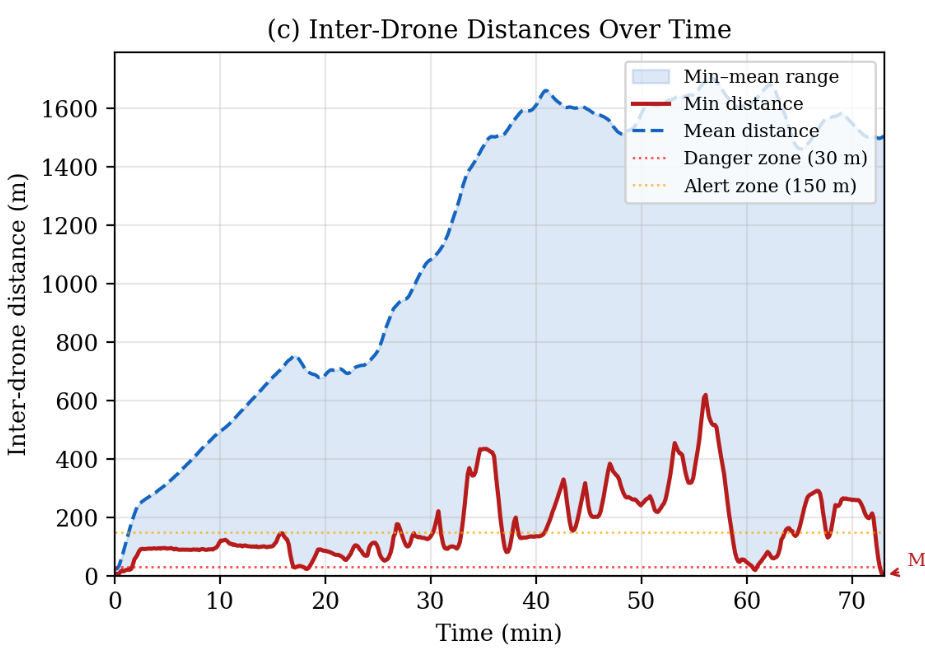
\includegraphics[width=0.9\textwidth]{images/9UAVs_inter_v2.png}
    \caption{Inter-drone distance plot for the swarm of 9 drones. The plot shows that the swarm is able to maintain safe distances between drones, with no instances of collisions or near-collisions.}
    \label{fig:9UAVs_between_drones_distance}
\end{figure}
